\documentclass{standalone}
\usepackage{tikz}
\usetikzlibrary{patterns, positioning}


\begin{document}
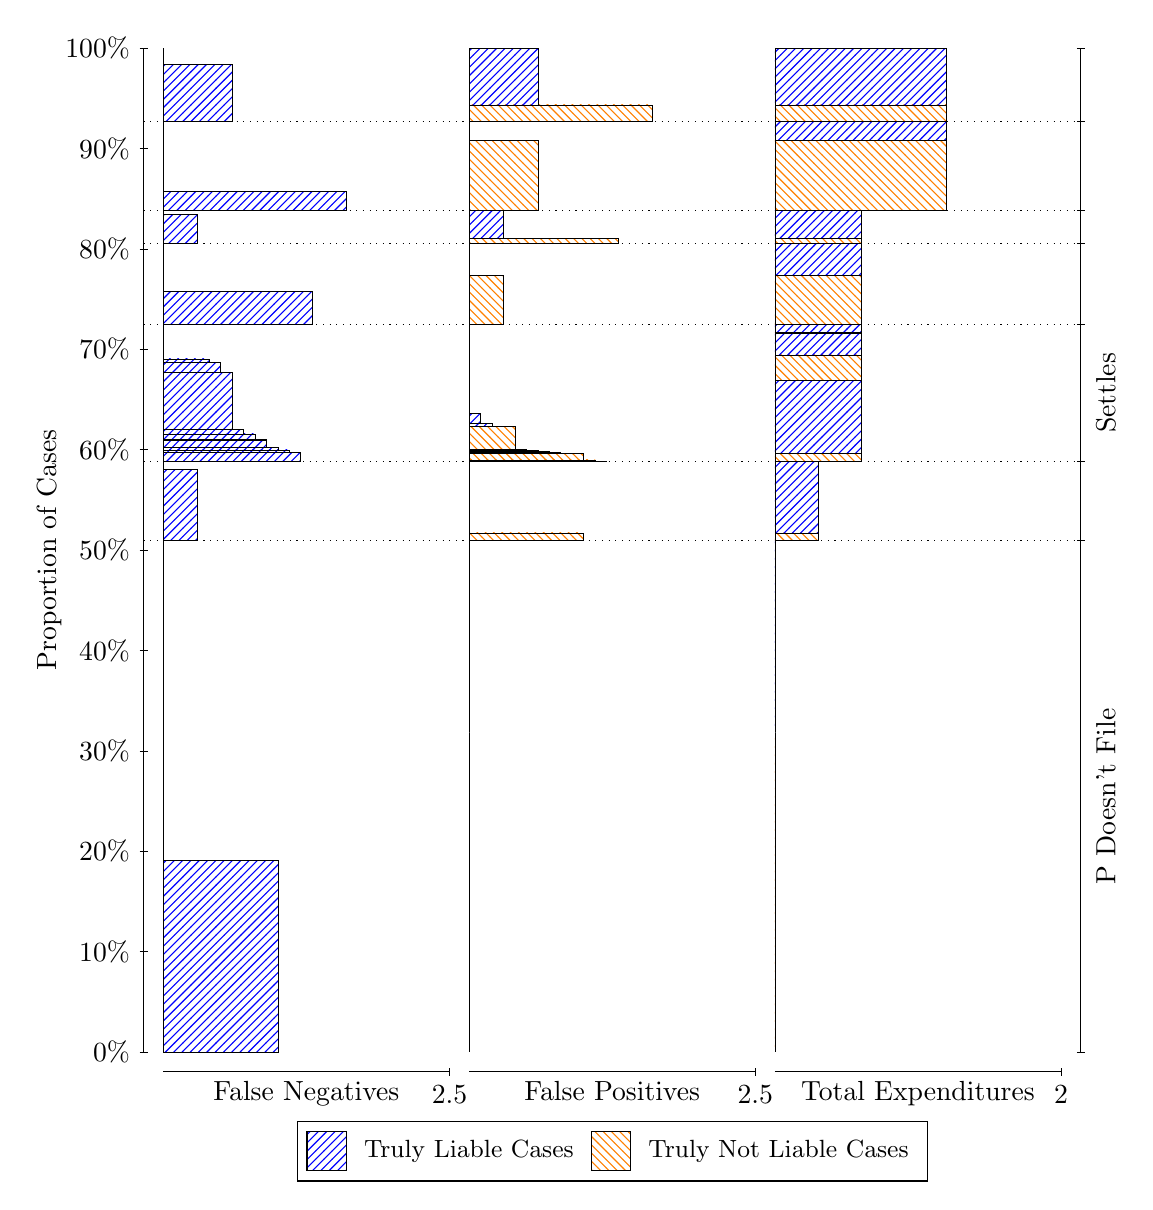
\begin{tikzpicture}
\draw[black, very thin] (1.5,1.75) -- (1.5,14.5);
\node[rotate=90, text=black, anchor=center] at (0.3, 8.125) {Proportion of Cases};
\draw[black, very thin] (1.45,1.75) -- (1.55,1.75);
\node[text=black, anchor=east] at (1.45, 1.75) {0\%};
\draw[black, very thin] (1.45,3.025) -- (1.55,3.025);
\node[text=black, anchor=east] at (1.45, 3.025) {10\%};
\draw[black, very thin] (1.45,4.3) -- (1.55,4.3);
\node[text=black, anchor=east] at (1.45, 4.3) {20\%};
\draw[black, very thin] (1.45,5.575) -- (1.55,5.575);
\node[text=black, anchor=east] at (1.45, 5.575) {30\%};
\draw[black, very thin] (1.45,6.85) -- (1.55,6.85);
\node[text=black, anchor=east] at (1.45, 6.85) {40\%};
\draw[black, very thin] (1.45,8.125) -- (1.55,8.125);
\node[text=black, anchor=east] at (1.45, 8.125) {50\%};
\draw[black, very thin] (1.45,9.4) -- (1.55,9.4);
\node[text=black, anchor=east] at (1.45, 9.4) {60\%};
\draw[black, very thin] (1.45,10.675) -- (1.55,10.675);
\node[text=black, anchor=east] at (1.45, 10.675) {70\%};
\draw[black, very thin] (1.45,11.95) -- (1.55,11.95);
\node[text=black, anchor=east] at (1.45, 11.95) {80\%};
\draw[black, very thin] (1.45,13.225) -- (1.55,13.225);
\node[text=black, anchor=east] at (1.45, 13.225) {90\%};
\draw[black, very thin] (1.45,14.5) -- (1.55,14.5);
\node[text=black, anchor=east] at (1.45, 14.5) {100\%};

\draw[black, very thin] (13.4,1.75) -- (13.4,14.5);
\draw[black, very thin] (13.35,1.75) -- (13.45,1.75);
\node[anchor=west] at (13.35, 1.75) {};
\draw[black, very thin] (13.35,8.2425) -- (13.45,8.2425);
\node[anchor=west] at (13.35, 8.2425) {};
\draw[black, very thin] (13.35,9.2482) -- (13.45,9.2482);
\node[anchor=west] at (13.35, 9.2482) {};
\draw[black, very thin] (13.35,10.994) -- (13.45,10.994);
\node[anchor=west] at (13.35, 10.994) {};
\draw[black, very thin] (13.35,12.022) -- (13.45,12.022);
\node[anchor=west] at (13.35, 12.022) {};
\draw[black, very thin] (13.35,12.441) -- (13.45,12.441);
\node[anchor=west] at (13.35, 12.441) {};
\draw[black, very thin] (13.35,13.566) -- (13.45,13.566);
\node[anchor=west] at (13.35, 13.566) {};
\draw[black, very thin] (13.35,14.5) -- (13.45,14.5);
\node[anchor=west] at (13.35, 14.5) {};

\draw[black, very thin, pattern color=blue, pattern=north east lines] (1.75,1.75) rectangle (3.2033,4.1836);
\draw[black, very thin, pattern color=orange, pattern=north west lines] (1.75,4.1836) rectangle (1.75,8.2425);
\draw[black, very thin, pattern color=blue, pattern=north east lines] (1.75,8.2425) rectangle (2.186,9.1495);
\draw[black, very thin, pattern color=orange, pattern=north west lines] (1.75,9.1495) rectangle (1.75,9.2482);
\draw[black, very thin, pattern color=blue, pattern=north east lines] (1.75,9.2482) rectangle (3.494,9.3645);
\draw[black, very thin, pattern color=blue, pattern=north east lines] (1.75,9.3645) rectangle (3.3487,9.3961);
\draw[black, very thin, pattern color=blue, pattern=north east lines] (1.75,9.3961) rectangle (3.2033,9.4316);
\draw[black, very thin, pattern color=blue, pattern=north east lines] (1.75,9.4316) rectangle (3.058,9.5181);
\draw[black, very thin, pattern color=blue, pattern=north east lines] (1.75,9.5181) rectangle (3.058,9.5282);
\draw[black, very thin, pattern color=blue, pattern=north east lines] (1.75,9.5282) rectangle (2.9127,9.5997);
\draw[black, very thin, pattern color=blue, pattern=north east lines] (1.75,9.5997) rectangle (2.7673,9.6546);
\draw[black, very thin, pattern color=blue, pattern=north east lines] (1.75,9.6546) rectangle (2.622,10.379);
\draw[black, very thin, pattern color=blue, pattern=north east lines] (1.75,10.379) rectangle (2.4767,10.509);
\draw[black, very thin, pattern color=blue, pattern=north east lines] (1.75,10.509) rectangle (2.3313,10.551);
\draw[black, very thin, pattern color=orange, pattern=north west lines] (1.75,10.551) rectangle (1.75,10.994);
\draw[black, very thin, pattern color=blue, pattern=north east lines] (1.75,10.994) rectangle (3.6393,11.405);
\draw[black, very thin, pattern color=orange, pattern=north west lines] (1.75,11.405) rectangle (1.75,12.022);
\draw[black, very thin, pattern color=blue, pattern=north east lines] (1.75,12.022) rectangle (2.186,12.385);
\draw[black, very thin, pattern color=orange, pattern=north west lines] (1.75,12.385) rectangle (1.75,12.441);
\draw[black, very thin, pattern color=blue, pattern=north east lines] (1.75,12.441) rectangle (4.0753,12.677);
\draw[black, very thin, pattern color=orange, pattern=north west lines] (1.75,12.677) rectangle (1.75,13.566);
\draw[black, very thin, pattern color=blue, pattern=north east lines] (1.75,13.566) rectangle (2.622,14.289);
\draw[black, very thin, pattern color=orange, pattern=north west lines] (1.75,14.289) rectangle (1.75,14.5);
\draw[black, very thin, pattern color=orange, pattern=north west lines] (5.6333,1.75) rectangle (5.6333,5.8089);
\draw[black, very thin, pattern color=blue, pattern=north east lines] (5.6333,5.8089) rectangle (5.6333,8.2425);
\draw[black, very thin, pattern color=orange, pattern=north west lines] (5.6333,8.2425) rectangle (7.0867,8.3412);
\draw[black, very thin, pattern color=blue, pattern=north east lines] (5.6333,8.3412) rectangle (5.6333,9.2482);
\draw[black, very thin, pattern color=orange, pattern=north west lines] (5.6333,9.2482) rectangle (7.3773,9.2532);
\draw[black, very thin, pattern color=orange, pattern=north west lines] (5.6333,9.2532) rectangle (7.232,9.2691);
\draw[black, very thin, pattern color=orange, pattern=north west lines] (5.6333,9.2691) rectangle (7.0867,9.3496);
\draw[black, very thin, pattern color=orange, pattern=north west lines] (5.6333,9.3496) rectangle (6.9413,9.3567);
\draw[black, very thin, pattern color=orange, pattern=north west lines] (5.6333,9.3567) rectangle (6.796,9.3664);
\draw[black, very thin, pattern color=orange, pattern=north west lines] (5.6333,9.3664) rectangle (6.6507,9.3795);
\draw[black, very thin, pattern color=orange, pattern=north west lines] (5.6333,9.3795) rectangle (6.5053,9.3893);
\draw[black, very thin, pattern color=orange, pattern=north west lines] (5.6333,9.3893) rectangle (6.36,9.4037);
\draw[black, very thin, pattern color=orange, pattern=north west lines] (5.6333,9.4037) rectangle (6.2147,9.6915);
\draw[black, very thin, pattern color=blue, pattern=north east lines] (5.6333,9.6915) rectangle (5.924,9.7336);
\draw[black, very thin, pattern color=blue, pattern=north east lines] (5.6333,9.7336) rectangle (5.7787,9.8638);
\draw[black, very thin, pattern color=blue, pattern=north east lines] (5.6333,9.8638) rectangle (5.6333,10.994);
\draw[black, very thin, pattern color=orange, pattern=north west lines] (5.6333,10.994) rectangle (6.0693,11.611);
\draw[black, very thin, pattern color=blue, pattern=north east lines] (5.6333,11.611) rectangle (5.6333,12.022);
\draw[black, very thin, pattern color=orange, pattern=north west lines] (5.6333,12.022) rectangle (7.5227,12.078);
\draw[black, very thin, pattern color=blue, pattern=north east lines] (5.6333,12.078) rectangle (6.0693,12.441);
\draw[black, very thin, pattern color=orange, pattern=north west lines] (5.6333,12.441) rectangle (6.5053,13.33);
\draw[black, very thin, pattern color=blue, pattern=north east lines] (5.6333,13.33) rectangle (5.6333,13.566);
\draw[black, very thin, pattern color=orange, pattern=north west lines] (5.6333,13.566) rectangle (7.9587,13.778);
\draw[black, very thin, pattern color=blue, pattern=north east lines] (5.6333,13.778) rectangle (6.5053,14.5);
\draw[black, very thin, pattern color=orange, pattern=north west lines] (9.5167,1.75) rectangle (9.5167,5.8089);
\draw[black, very thin, pattern color=blue, pattern=north east lines] (9.5167,5.8089) rectangle (9.5167,8.2425);
\draw[black, very thin, pattern color=orange, pattern=north west lines] (9.5167,8.2425) rectangle (10.062,8.3412);
\draw[black, very thin, pattern color=blue, pattern=north east lines] (9.5167,8.3412) rectangle (10.062,9.2482);
\draw[black, very thin, pattern color=orange, pattern=north west lines] (9.5167,9.2482) rectangle (10.607,9.3542);
\draw[black, very thin, pattern color=blue, pattern=north east lines] (9.5167,9.3542) rectangle (10.607,10.28);
\draw[black, very thin, pattern color=orange, pattern=north west lines] (9.5167,10.28) rectangle (10.607,10.604);
\draw[black, very thin, pattern color=blue, pattern=north east lines] (9.5167,10.604) rectangle (10.607,10.873);
\draw[black, very thin, pattern color=orange, pattern=north west lines] (9.5167,10.873) rectangle (10.607,10.887);
\draw[black, very thin, pattern color=blue, pattern=north east lines] (9.5167,10.887) rectangle (10.607,10.994);
\draw[black, very thin, pattern color=orange, pattern=north west lines] (9.5167,10.994) rectangle (10.607,11.611);
\draw[black, very thin, pattern color=blue, pattern=north east lines] (9.5167,11.611) rectangle (10.607,12.022);
\draw[black, very thin, pattern color=orange, pattern=north west lines] (9.5167,12.022) rectangle (10.607,12.078);
\draw[black, very thin, pattern color=blue, pattern=north east lines] (9.5167,12.078) rectangle (10.607,12.441);
\draw[black, very thin, pattern color=orange, pattern=north west lines] (9.5167,12.441) rectangle (11.697,13.33);
\draw[black, very thin, pattern color=blue, pattern=north east lines] (9.5167,13.33) rectangle (11.697,13.566);
\draw[black, very thin, pattern color=orange, pattern=north west lines] (9.5167,13.566) rectangle (11.697,13.778);
\draw[black, very thin, pattern color=blue, pattern=north east lines] (9.5167,13.778) rectangle (11.697,14.5);
\draw[black, dotted] (1.5,8.2425) -- (13.4,8.2425);
\draw[black, dotted] (1.5,9.2482) -- (13.4,9.2482);
\draw[black, dotted] (1.5,10.994) -- (13.4,10.994);
\draw[black, dotted] (1.5,12.022) -- (13.4,12.022);
\draw[black, dotted] (1.5,12.441) -- (13.4,12.441);
\draw[black, dotted] (1.5,13.566) -- (13.4,13.566);
\draw[black, very thin] (1.75,1.5) -- (5.3833,1.5);
\node[text=black, anchor=north] at (3.5667, 1.5) {False Negatives};
\draw[black, very thin] (5.3833,1.45) -- (5.3833,1.55);
\node[text=black, anchor=north] at (5.3833, 1.45) {2.5};

\draw[black, very thin] (5.6333,1.5) -- (9.2667,1.5);
\node[text=black, anchor=north] at (7.45, 1.5) {False Positives};
\draw[black, very thin] (9.2667,1.45) -- (9.2667,1.55);
\node[text=black, anchor=north] at (9.2667, 1.45) {2.5};

\draw[black, very thin] (9.5167,1.5) -- (13.15,1.5);
\node[text=black, anchor=north] at (11.333, 1.5) {Total Expenditures};
\draw[black, very thin] (13.15,1.45) -- (13.15,1.55);
\node[text=black, anchor=north] at (13.15, 1.45) {2};

\node[text=black, centered, rotate=90] at (13.72, 4.9962) {P Doesn't File};

\node[text=black, centered, rotate=90] at (13.72, 10.121) {Settles};





\draw (7.449999999999999,1.5) node[draw=none] (baseCoordinate) {};
\begin{scope}[align=center]
        \matrix[scale=0.5, draw=black, below=0.5cm of baseCoordinate, nodes={draw}, column sep=0.1cm]{
            \node[rectangle, draw, minimum width=0.5cm, minimum height=0.5cm, pattern color=blue, pattern=north east lines] {}; &
            \node[draw=none, font=\small, text=black] (B) {Truly Liable Cases}; &
            \node[rectangle, draw, minimum width=0.5cm, minimum height=0.5cm, pattern color=orange, pattern=north west lines] {}; &
            \node[draw=none, font=\small, text=black] (B) {Truly Not Liable Cases}; \\
            };
\end{scope}

\end{tikzpicture}
\end{document}